%
% tested with pdflatex (direct dvi -> pdf)
%
\documentclass[12pt,a4paper]{article}
%
%%%%% MAIN DEFINITIONS START - MODIFY AS NECESSARY

%%% Select the language (default English):
\def\mylang{e} % English
%\def\mylang{f} % Finnish
%\def\mylang{s} % Swedish

\newcommand{\mycourse}{PHYS-E0412 --- Computational Physics}
\newcommand{\mytitle}{Two-dimensional site percolation with periodic \newline boundary conditions}
\newcommand{\mypagenum}{iv+20+IV}
\newcommand{\mylanguage}{English}
\newcommand{\mypubdate}{January 30, 2020}
\newcommand{\mykeywords}{{}}

\newcommand{\myauthor}{Matias Haapalehto}
\newcommand{\mydegreeprog}{Engineering Physics and Mathematics}
\newcommand{\mymajor}{Engineering Physics}
\newcommand{\mymajorcode}{SCI3056}
\newcommand{\mysupervisor}{}
\newcommand{\myinstructor}{} % can be a list

%%%%% MAIN DEFINITIONS END
%
% package loadings

%\usepackage[finnish]{babel}         % set language to Finnish
%\usepackage{icomma}                 % intelligent comma for finnish language decimal separator
\usepackage[finnish,swedish,english]{babel} % set languages, start with English
\usepackage[utf8]{inputenc}          % input encoding to utf8
\usepackage[T1]{fontenc}             % fonts for umlauts
\usepackage{textcomp}                % highly recommend by psnfss2e.pdf
\usepackage{graphicx}                % the standard graphics package
\usepackage{siunitx}                 % provides the \SI{}{} -command.
\usepackage{url}                     % provides the badly needed \url{} -command
\usepackage[a4paper]{geometry}       % set the output page size
\usepackage{amsmath}                 % provides richer amount of mathematical symbols. [intlimits] -option makes integral limits as in blackboards.
\usepackage{amsfonts}                % provides richer amount of mathematical fonts
\usepackage{cite}                    % sorts citations like [30, 1, 31, 32, 3] into [1, 3, 30-32].
%\usepackage{fancyhdr}                % for fancy headers
%\usepackage{flafter}                % makes all floats not to be placed in the before their declaration.
\usepackage[small]{caption}          % caption text fine tuning
%\usepackage{array}                  % provides more tabular options
\usepackage{rotating}                % provides the \sidewaystable{} -command and other rotations
\usepackage[version=3]{mhchem}       % provides nuclide and other related commands (\ce)
\usepackage{tikz}                    % provides correctly working circled letters and other plotting commands
\usepackage{subfigure}               % provides the \subfigure -command, is actually obsolute so consider using ctable figures.
\usepackage{ae}                      % some font thingies
\usepackage{ctable}                  % fine tuned tables, http://www.ctan.org/tex-archive/macros/latex/contrib/ctable/
\usepackage{multirow}                % spanning multiple rows in tables
\usepackage{verbatim}                % comments'
\usepackage{printlen}                % to print lengths of some things
\usepackage[normalem]{ulem}          % for \s[trike]out command to be used with DONE -command.
\usepackage{hyperref}                % yet another package. [import as the last one to avoid collisions with redefinitions]
\usepackage[dmyyyy]{datetime}        % alternative \today output.
\usepackage{dcolumn}                 % tabular columns alignment, e.g., along the decimal point

% hyperref
\hypersetup{
colorlinks = {true}, % color or boxlinks --- keep it true.
linkcolor = {black},
anchorcolor = {black},
citecolor = {black},
menucolor = {black},
filecolor = {black},
urlcolor = {blue},
runcolor = {black},
linkbordercolor = {black},
citebordercolor = {black},
urlbordercolor = {black},
menubordercolor = {black},
filebordercolor = {black},
runbordercolor = {black},
linktoc = {all},
pdftitle = {\mytitle},
pdfpagelayout = {SinglePage},
pdfauthor = {\myauthor},
pdfkeywords = \mykeywords,
pdfstartview = {Fit},
unicode = {true},
}
\def\sectionautorefname{Section}
\def\appendixautorefname{App.}


% tikz
\usetikzlibrary{%
  arrows,shapes,positioning,chains,scopes,shadows,topaths%
  %shadings,%
  %calc,%
  %fit%,%
  %patterns,%
  %plotmarks,%
  %positioning,%
  %shapes.geometric,%
  %shapes.misc,%
  %shapes.symbols,%
  %shapes.arrows,%
  %shapes.callouts,%
  %shapes.multipart,%
  %shapes.gates.logic.US,%
  %shapes.gates.logic.IEC,%
  %er,%
  %automata,%
  %backgrounds,%
  %chains,%
  %trees,%
  %petri,%
  %mindmap,%
  %matrix,%
  %calendar,%
  %folding,%
  %fadings,%
  %through,%
  %scopes,%
  %decorations.fractals,%
  %decorations.shapes,%
  %decorations.text,%
  %decorations.pathmorphing,%
  %decorations.pathreplacing,%
  %decorations.footprints,%
  %decorations.markings,%
} 

% datetime
\renewcommand{\dateseparator}{.}

% make the text height about 2 cm larger than default
\setlength{\textheight}{45\baselineskip}

% tabular columns alignment along the decimal point
\newcolumntype{d}[1]{D{.}{.}{#1}}

% newly defined commands

% sensible positions for floats (figures and tables)
\renewcommand{\floatpagefraction}{0.90}
\renewcommand{\topfraction}{1.0}
\renewcommand{\bottomfraction}{1.0}
\renewcommand{\textfraction}{0.0}
\setcounter{topnumber}{10}
\setcounter{bottomnumber}{10}
\setcounter{totalnumber}{10}

% a set of commonly usable commands
\newcounter{todono}
\setcounter{todono}{0}
\newcommand{\TODO}[1]{\addtocounter{todono}{1}\emph{TODO~\arabic{todono}: #1}}
\newcommand{\DONE}[1]{\addtocounter{todono}{1}\emph{\sout{TODO~\arabic{todono}: #1}}}
\newcommand{\note}[1]{\texttt{[ #1 ]}}
%\newcommand{\comment}[1]{\note{#1}}

% in case arrow -over vectors get ugly
\renewcommand{\vec}[1]{\mathbf{\bar{#1}}} % symbolic physical vectors
\newcommand{\unitvec}[1]{\mathbf{\hat{#1}}} % symbolic physical unit vectors
\newcommand{\matvec}[1]{\mathbf{#1}} % symbolic mathematical vectors
\newcommand{\mat}[1]{\mathbf{#1}} % symbolic matrixes

% circled text correctly
\renewcommand*\textcircled[1]{\tikz[baseline=(char.base)]{\node[shape=circle,draw,inner sep=2pt] (char) {#1};}}

% k-eff and k-inf
\newcommand{\keff}[0]{\ensuremath{k_{\textnormal{eff}}}}
\newcommand{\kinf}[0]{\ensuremath{k_{\infty}}}

% laplace -operator
\newcommand{\laplace}[0]{\ensuremath{\Delta}}

% programs
\newcommand{\casmof}[0]{\texttt{CASMO-4}}
\newcommand{\casmo}[0]{\texttt{CASMO-4E}}
\newcommand{\cmslink}[0]{\texttt{CMS-LINK}}
\newcommand{\simulate}[0]{\texttt{SIMULATE-3}}
\newcommand{\serpent}[0]{\texttt{Serpent}}
\newcommand{\interpin}[0]{\texttt{INTERPIN}}
\newcommand{\njoy}[0]{\texttt{NJOY}}

% file types
\newcommand{\postscript}[0]{\texttt{PostScript}}
\newcommand{\dtfiv}[0]{\texttt{DTF-IV}}
\newcommand{\cccciv}[0]{\texttt{CCCC-IV}}
\newcommand{\matxs}[0]{\texttt{MATXS}}
\newcommand{\wims}[0]{\texttt{WIMS}}

% other wierdly written names
\newcommand{\qpanda}[0]{QPANDA}

% organizations
\newcommand{\iaea}[0]{IAEA}

% things that might be changed later
%\newcommand{\burnup}[0]{\ensuremath{\textnormal{Bu}}}
\newcommand{\burnup}[0]{\ensuremath{B}}

% integral substitution
\DeclareMathOperator*{\subs}{\textnormal{\Huge\bfseries\itshape|}}

% transpose mark
\newcommand{\transpose}{\mathrm{T}}

% footnote symbols for tables
\newcounter{fnc}
\newcommand{\foot}[1]{\setcounter{fnc}{#1}\ensuremath{\fnsymbol{fnc}}}

% modules
\newcommand{\reconr}[0]{\texttt{RECONR}}
\newcommand{\broadr}[0]{\texttt{BROADR}}
\newcommand{\unresr}[0]{\texttt{UNRESR}}
\newcommand{\heatr}[0]{\texttt{HEATR}}
\newcommand{\thermr}[0]{\texttt{THERMR}}
\newcommand{\groupr}[0]{\texttt{GROUPR}}
\newcommand{\gaminr}[0]{\texttt{GAMINR}}
\newcommand{\errorr}[0]{\texttt{ERRORR}}
\newcommand{\covr}[0]{\texttt{COVR}}
\newcommand{\moder}[0]{\texttt{MODER}}
\newcommand{\dtfr}[0]{\texttt{DTFR}}
\newcommand{\ccccr}[0]{\texttt{CCCCR}}
\newcommand{\matxsr}[0]{\texttt{MATXSR}}
\newcommand{\resxsr}[0]{\texttt{RESXSR}}
\newcommand{\acer}[0]{\texttt{ACER}}
\newcommand{\powr}[0]{\texttt{POWR}}
\newcommand{\wimsr}[0]{\texttt{WIMSR}}
\newcommand{\plotr}[0]{\texttt{PLOTR}}
\newcommand{\viewr}[0]{\texttt{VIEWR}}
\newcommand{\mixr}[0]{\texttt{MIXR}}
\newcommand{\purr}[0]{\texttt{PURR}}
\newcommand{\leapr}[0]{\texttt{LEAPR}}
\newcommand{\gaspr}[0]{\texttt{GASPR}}

% tape types
\newcommand{\ace}[0]{\texttt{ACE}}
\newcommand{\sixthendf}[0]{\texttt{ENDF-6}}
\newcommand{\pendf}[0]{\texttt{PENDF}}
\newcommand{\gendf}[0]{\texttt{GENDF}}
\newcommand{\errorrformat}[0]{\texttt{kovarianssitiedosto}}
\newcommand{\boxer}[0]{\texttt{BOXER}}

% definitions in lab instructions
\newcommand{\cdeg}{\textdegree C}
\newcommand{\SHAMAN}{{\slshape SHA\-MAN\/}}
\newcommand{\UniSampo}{{\slshape Uni\-SAM\-PO}}
\newcommand{\UniSAMPO}{{\slshape Uni\-SAM\-PO}}
\newcommand{\finnrepo}{TKK-F-C111}
\newcommand{\FiR}{FiR~1}
\newcommand{\tm}{$^\textrm{TM}$}
\newcommand{\ubar}[1]{\underline{#1}}
\newcommand{\tenexp}[1]{\times 10^{#1}}

%
\begin{document}
%
\if\mylang f
\selectlanguage{finnish}
\fi
\if\mylang s
\selectlanguage{swedish}
\fi
%
\pagenumbering{roman}
% the cover page
\begin{titlepage}
%\enlargethispage{10mm}

{\sffamily

\if\mylang e

\noindent
\fontsize{12}{14}\selectfont
Aalto University \newline
School of Science \newline
%Department of Applied Physics

\vspace{40mm}

\noindent
\fontsize{14}{16}\selectfont
\myauthor

\vspace{10mm}

\noindent
\fontsize{18}{22}\selectfont
\textbf{\mytitle}

\vspace{90mm}

\noindent
\fontsize{12}{14}\selectfont
Course project report \\[4mm]
\mycourse \\[4mm]
Report submitted : \mypubdate \\[4mm]
%\mbox{}\\[4mm]
%\makebox[25mm][l]{Supervisor:} \mysupervisor \\[4mm]
%\makebox[25mm][l]{Instructor(s):} \myinstructor

\fi

\if\mylang f

\noindent
\fontsize{12}{14}\selectfont
Aalto-yliopisto \newline
Perustieteiden korkeakoulu \newline
Teknillisen fysiikan laitos

\vspace{40mm}

\noindent
\fontsize{14}{16}\selectfont
\myauthor

\vspace{10mm}

\noindent
\fontsize{18}{22}\selectfont
\textbf{\mytitle}

\vspace{90mm}

\noindent
\fontsize{12}{14}\selectfont
Erikoistyöraportti \\[4mm]
\mycourse \\[4mm]
Raportti lähetetty hyväksyttäväksi: \mypubdate \\[4mm]
\mbox{}\\[4mm]
\makebox[25mm][l]{Valvoja:} \mysupervisor \\[4mm]
\makebox[25mm][l]{Ohjaaja(t):} \myinstructor

\fi

\if\mylang s

\noindent
\fontsize{12}{14}\selectfont
Aalto-universitetet \newline
Högskolan för teknikvetenskaper \newline
Institutionen för teknisk fysik

\vspace{40mm}

\noindent
\fontsize{14}{16}\selectfont
\myauthor

\vspace{10mm}

\noindent
\fontsize{18}{22}\selectfont
\textbf{\mytitle}

\vspace{90mm}

\noindent
\fontsize{12}{14}\selectfont
Specialarbeterapport \\[4mm]
\mycourse \\[4mm]
Rapport avsänd för godkännande: \mypubdate \\[4mm]
\mbox{}\\[4mm]
\makebox[25mm][l]{Övervakare:} \mysupervisor \\[4mm]
\makebox[25mm][l]{Handledare:} \myinstructor

\fi

} % end of \sffamily

\end{titlepage}

%\newpage

%\thispagestyle{empty}
%\mbox{}

\newpage

%\clearpage
%\setcounter{page}{2}
%\thispagestyle{empty}
%%%% Edit ONLY the abstract text block that corresponds to the language!

{\sffamily

\noindent
\if\mylang e

\includegraphics[height=30mm]{Aalto_SCI_EN}
\fi
\if\mylang f

\includegraphics[height=30mm]{Aalto_SCI_FI}
\fi
\if\mylang s

\includegraphics[height=30mm]{Aalto_SCI_SE}
\fi

\vspace*{-21mm}

{\small
{\bfseries
\if\mylang e
\begin{tabular*}{105mm}{lr}
\multicolumn{1}{l}{\mbox{}\hspace{65mm}\mbox{}}
& \textcolor{gray}{Aalto University, P.O. BOX 11000, 00076 AALTO} \\
& \textcolor{gray}{www.aalto.fi} \\
& Abstract of Physics Special Assignment \\
\end{tabular*}
\fi
\if\mylang f
\begin{tabular*}{105mm}{lr}
\multicolumn{1}{l}{\mbox{}\hspace{80mm}\mbox{}}
& \textcolor{gray}{Aalto-yliopisto, PL 11000, 00076 AALTO} \\
& \textcolor{gray}{www.aalto.fi} \\
& Fysiikan erikoistyön tiivistelmä \\
\end{tabular*}
\fi
\if\mylang s
\begin{tabular*}{105mm}{lr}
\multicolumn{1}{l}{\mbox{}\hspace{70mm}\mbox{}}
& \textcolor{gray}{Aalto-universitetet, PB 11000, 00076 AALTO} \\
& \textcolor{gray}{www.aalto.fi} \\
& Sammandrag av specialarbete i fysik \\
\end{tabular*}
\fi
}
}

\vspace*{10mm}

\if\mylang e
\begin{tabular*}{160mm}{lll}
\hline
\multicolumn{3}{l}{\textbf{Author} \myauthor} \\[1mm] \hline
\multicolumn{3}{l}{\textbf{Title of the work} \mytitle}  \\[1mm] \hline
\multicolumn{3}{l}{\textbf{Degree programme} \mydegreeprog} \\[1mm] \hline
\multicolumn{2}{l}{\textbf{Major} \mymajor} &
\textbf{Code of major} \mymajorcode \\[1mm] \hline
\multicolumn{3}{l}{\textbf{Supervisor} \mysupervisor} \\[1mm] \hline
\multicolumn{3}{l}{\textbf{Instructor(s)} \myinstructor} \\[1mm] \hline
\textbf{Date} \mypubdate &
\textbf{Number of pages} \mypagenum &
\textbf{Language} \mylanguage \\[1mm] \hline \\[1mm]
\textbf{Abstract} \\[1mm]
\multicolumn{3}{p{155mm}}{%
%%%
%%% START ABSTRACT TEXT (ENGLISH REPORT)
%%%
We derive a formalism to order nuclides by their importance to a given quantity of 
interest. A quantity can be any result of any linear effect of nuclides. Linear effects 
yield quantities that depend linearly on the amounts of nuclides, such as decay heat 
emission rate, spontaneous fission rate and neutron balance rate. Non-linear effects yield 
quantities such as effective multiplication factor and detectability of nuclides, and 
depend non-linearly on the amounts of nuclides.

The formalism can be used in identification of important minority and majority nuclides 
for any application. Application-specific criteria must be expressed as quantities of 
interest for which effects must be derived. This part remains to be an art. The formalism 
can be used to order nuclides by their importance to selected quantities of interest. 
Another art is to judge which nuclide is the last important one for a quantity: any 
nuclide with less importance is not important.

Suitable criteria, expressed as quantities of interest, are presented for three 
applications: reactor performance, radioactive waste storage and proliferation resistance. 
For illustration, the formalism is applied to a case of radioactive waste storage of a 
high burnup BWR assembly.
%%%
%%% END ABSTRACT TEXT
%%%
}
\\[1mm] \hline
\multicolumn{3}{l}{\textbf{Keywords} \mykeywords} \\[1mm] \hline
\end{tabular*}
\fi

\if\mylang f
\begin{tabular*}{160mm}{lll}
\hline
\multicolumn{3}{l}{\textbf{Tekijä} \myauthor} \\[1mm] \hline
\multicolumn{3}{l}{\textbf{Työn nimi} \mytitle}  \\[1mm] \hline
\multicolumn{3}{l}{\textbf{Koulutusohjelma} \mydegreeprog} \\[1mm] \hline
\multicolumn{2}{l}{\textbf{Pääaine} \mymajor} &
\textbf{Pääaineen koodi} \mymajorcode \\[1mm] \hline
\multicolumn{3}{l}{\textbf{Työn valvoja} \mysupervisor} \\[1mm] \hline
\multicolumn{3}{l}{\textbf{Työn ohjaaja(t)} \myinstructor} \\[1mm] \hline
\textbf{Päivämäärä} \mypubdate &
\textbf{Sivumäärä} \mypagenum &
\textbf{Kieli} \mylanguage \\[1mm] \hline
\textbf{Tiivistelmä} \\[1mm] \\[1mm]
\multicolumn{3}{p{155mm}}{%
%%%
%%% START ABSTRACT TEXT (FINNISH REPORT)
%%%
Tähän kirjoitetaan suomenkielisen erikoistyön tiivistelmä.
%%%
%%% END ABSTRACT TEXT
%%%
}
\\[1mm] \hline
\multicolumn{3}{l}{\textbf{Avainsanat} \mykeywords} \\[1mm] \hline
\end{tabular*}
\fi

\if\mylang s
\begin{tabular*}{160mm}{lll}
\hline
\multicolumn{3}{l}{\textbf{Författare} \myauthor} \\[1mm] \hline
\multicolumn{3}{l}{\textbf{Titel} \mytitle}  \\[1mm] \hline
\multicolumn{3}{l}{\textbf{Examensprogram} \mydegreeprog} \\[1mm] \hline
\multicolumn{2}{l}{\textbf{Huvudämne} \mymajor} &
\textbf{Huvudämnets kod} \mymajorcode \\[1mm] \hline
\multicolumn{3}{l}{\textbf{Ansvarig lärare} \mysupervisor} \\[1mm] \hline
\multicolumn{3}{l}{\textbf{Handledare} \myinstructor} \\[1mm] \hline
\textbf{Datum} \mypubdate &
\textbf{Sidantal} \mypagenum &
\textbf{Språk} \mylanguage \\[1mm] \hline
\textbf{Sammandrag} \\[1mm] \\[1mm]
\multicolumn{3}{p{155mm}}{%
%%%
%%% START ABSTRACT TEXT (SWEDISH REPORT)
%%%
Här är platsen för sammandrag av ett svenskt specialarbete.
%%%
%%% END ABSTRACT TEXT
%%%
}
\\[1mm] \hline
\multicolumn{3}{l}{\textbf{Nyckelord} \mykeywords} \\[1mm] \hline
\end{tabular*}
\fi

} % end of \sffamily

%\clearpage
%% the table of contents page
\thispagestyle{empty}
\tableofcontents

%\clearpage
%
\pagenumbering{arabic}
\setcounter{page}{1}


\section{Background}

The statement of site percolation is quite simple: every site in a lattice is either occupied with a probability $p$ or not with probability $1-p$. Neighboring occupied sites are grouped into clusters. At a specific value of $p$, we can observe an interesting phenomenon: the formation of a cluster spanning the entire system. This is called percolation. In the limit of an infinite lattice, there is a finite threshold probability $p_c$ such that~\cite{Gould_2006}:
\begin{itemize}
	\item for $p < p_c$ no spanning cluster exists and all clusters are finite
	\item for $p > p_c$ a spanning cluster exists
	\item for $p = p_c$ a spanning cluster exists with a finite probability larger than zero and less than one.
\end{itemize}
No exact results are known for the percolation threshold of a square lattice, which makes the problem an interesting model to solve computationally.

The model originates from studies in percolation in materials such as rock or concrete~\cite{Newman_2001}. Other applications outside physics include modeling resistor networks or forest fires~\cite{Newman_2001}. 


\section{Theory and methodology}
The percolation threshold is defined as the site occupation probability at which a spanning cluster first appears in an infinite lattice~\cite{Gould_2006}. Since we can only simulate a finite lattice, we must choose a definition of the spanning cluster. For example, we can define it as a cluster that (i) spans the lattice either horizontally or vertically, (ii) spans the lattice in a fixed direction, (iii) spans the lattice both horizontally or vertically or (iv) spans the lattice only in one direction. The value of $p_c$ depends also on the type of lattice and its dimension. The lattice we use in this study is the two-dimensional square lattice, where each site has four nearest neighbors.

In our simulation, we want to estimate an observable quantity over a range of values of $p$. Now we would have to repeat the simulation at many values of $p$, which makes the computation slow. Instead, it is faster to measure the observable for fixed numbers of occupied sites in the range of interest~\cite{Newman_2001}. Let us refer to the ensemble of states of a system with $n$ occupied sites as the \emph{microcanonical percolation ensemble}. On the other hand, the case where the occupation probability $p$ is fixed is called the \emph{canonical percolation ensemble}. In the canonical ensemble, the probability of there being exactly $n$ occupied sites is given by the binomial distribution:
\begin{align}
B(N, n, p) = {N \choose n}p^n(1-p)^{N-n}
\end{align}   
Where $N$ is the total number of sites. Therefore, if we can measure the set of observables $Q_n$ within the microcanonical ensemble, then the value in the canonical ensemble is given by a convolution of the set of measurement with the binomial distribution:
\begin{align}
Q(p) = \sum_{n=0}^N B(N, n, p)Q_n = \sum_{n=0}^N{N \choose n}p^n(1-p)^{N-n}Q_n
\end{align}
Direct evaluation of the binomial coefficients using factorials is not possible, therefore we will use the following method. The binomial distribution reaches a maximum for a given $N$ when $n = n_max = pN$. We set this value to 1 for the time being. Then we compute the rest of the values of $B(N, n, p)$ iteratively using:
\begin{align}
B(N, n, p) = 
	\begin{cases}
	B(N, n-1, p)\frac{N-n+1}{n}\frac{p}{1-p}, &\quad n>n_{max}\\
	B(N, n+1, p)\frac{n+1}{N-n}\frac{1-p}{p}, &\quad n<n_{max}
	\end{cases}
\end{align}
Lastly, we normalize the distribution by dividing each value by the normalization constant $C = \sum_n B(N, n, p)$.

One observable of interest is the probability $R_L(p)$. This is defined as the probability, for a value of $p$, that there exists a cluster wrapping completely around a square lattice of linear dimension $L$ periodic boundary conditions. There are several possible ways in which wrapping can occur, and therefore multiple definition for $R_L$~\cite{Newman_2001}:
\begin{itemize}
	\item $R_L^{(h)}$ is the probability that there exists a cluster which wraps around the horizontal direction
	\item $R_L^{(e)}$ is the probability that there exists a cluster which wraps around either the horizontal or vertical direction, or both
	\item $R_L^{(b)}$ is the probability that there exists a cluster which wraps around both horizontal and vertical directions
	\item $R_L^{(1)}$ is the probability that there exists a cluster which wraps around either direction, but not both.
\end{itemize}
An example of a cluster wrapping in either direction is given in~\autoref{fig:grid64}.

\begin{figure}
	\centering
		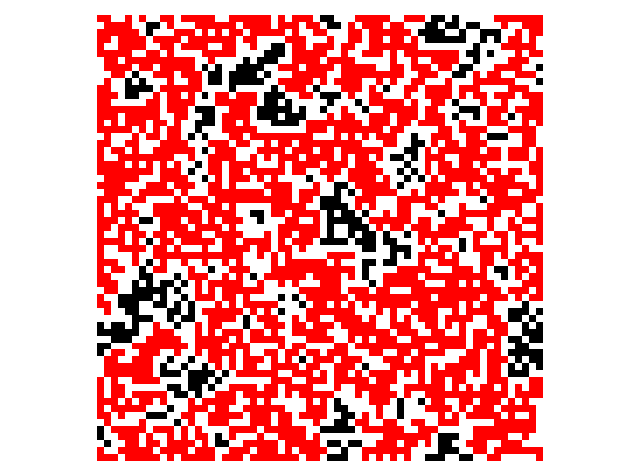
\includegraphics[height=80mm]{../plots/sample64}
		\caption{\label{fig:grid64} Sample lattice (L=64) where the spanning cluster is marked in red.}
\end{figure}

These probabilities satisfy the following equations:
\begin{align}
R_L^{(e)} &= 2R_L^{(h)}-R_L^{(b)}\\
R_L^{(1)} &= R_L^{(h)} -R_L^{(b)}
\end{align}
Therefore only two of them are independent. The reason we are interesting in the wrapping probabilities is that their values can be calculated exactly for an infinite lattice~\cite{Newman_2001}. The values to ten figures are given by:
\begin{align}
R^{(h)}_\infty(p_c) = 0.521058290\\
R^{(e)}_\infty(p_c) = 0.690473725\\
R^{(b)}_\infty(p_c) = 0.351642855\\
R^{(1)}_\infty(p_c) = 0.169415435
\end{align}
Now we can estimate $p_c$ as the solution $p$ of the following equation:
\begin{align}
R_L(p) =  R_\infty(p_c)
\end{align}
Our estimate of the mean of $R_L(p_c)$ over $n$ runs is drawn from the binomial distribution which has standard deviation:
\begin{align}
\sigma_{R_L} =\sqrt{\frac{R_L(p_c)[1-R_L(p_c)]}{n}}
\end{align}
We can evaluate the error by approximating $R_L(p_c)$ by the known value of $R_\infty(p_c)$. 
Ref.~\cite{Newman_2001} conjectures that $R_L(p_c)$ converges to $R_\infty(p_c)$ as $L^{-2}$. On the other hand, the width of the critical region decreases as $L^{-1/\nu}$, and therefore the gradient of $R_L(p)$ in the region goes as $L^{1/\nu}$. Thus the estimate of the critical occupation probability converges according to:
\begin{align}
p-p_c \sim L^{-2-1/\nu} = L^{-11/4}
\end{align}
Since for percolation on a square lattice we have $\nu = \frac 4 3$.

\subsection{Algorithm}

The Newman-Ziff algorithm was employed to simulate the system within the microcanonical ensemble.
The steps of the algorithm are as follows~\cite{Newman_2000}. The algorithm starts with an empty  lattice . As the lattice is populated in a random order, clusters are given a label identifying them. When a bond connecting two sites is added, they are either a member of the same cluster or they are members of two different clusters. In this second case, the labels need to be updated to reflect the fact that the bond has connected the clusters. 

In the interest of efficiency, the clusters are stored in an array mimicking a tree structure in which a site is chosen to be the "root" of the cluster. All other sites in the cluster point either to the cluster root or another site in the cluster. Starting from any site, the root node can be found by following these pointers. Clusters can be connected together by a adding a pointer from the root of one to the root of the other.

This type of algorithm is called \emph{weighted union–find with path compression}, weighted because the two trees are amalgamated by making the smaller a sub-tree of the other. Path compression signifies that the pointers of all traversed nodes are changed to point to the root node, in order to speed up the next searches. The steps taken to add one bond are roughly constant in time, therefore the algorithm adds N bonds in $\mathcal O(N)$ time.

In order find whether a configuration has percolated, additional work must be done. We add variables to each node which store the displacement to the parent node in both coordinates. Now the total displacement to the root node can be computed by traversing the tree and adding the displacements together. When a bond is added joining two sites $i$ and $j$ that are members of the same cluster, there are two paths from $i$ to the root node. One that goes through the parent of $i$ and another that consists of hopping to $j$ and then going through $j$'s parents. We sum the displacements along both of these paths, and percolation has occurred if the difference in displacement is equal to $\pm L$ in either of the coordinates~\cite{Mertens_2012}. 

The implementation of the algorithm was done in the C language, while Python libraries were used for the plots. The Mersenne Twister was the pseudo-random number generator employed. 

\section{Results from simulations}
The number of Monte Carlo samples simulated for each value of $L$ is given in~\autoref{table:samples}.
The results for the wrapping probabilities are given in~\autoref{fig:plot1} and results of the finite size scaling estimation are given in~\autoref{fig:plot2}. Results for the percolation threshold estimates are given in~\autoref{table:pc}. The error was estimated using the variance of the linear regression.

\begin{table}[!htbp]
	\centering
		\begin{tabular}{ll}
		$L$ & $n$           \\
		32  & $10^9$        \\
		64  & $2\cdot 10^8$ \\
		128 & $5\cdot 10^7$ \\
		256 & $10^7$       	
		\end{tabular}
	\caption{\label{table:samples} Number of simulated Monte Carlo samples $n$ for each value of the linear dimension $L$ of the square lattice}
\end{table}

\begin{figure}
	\centering
		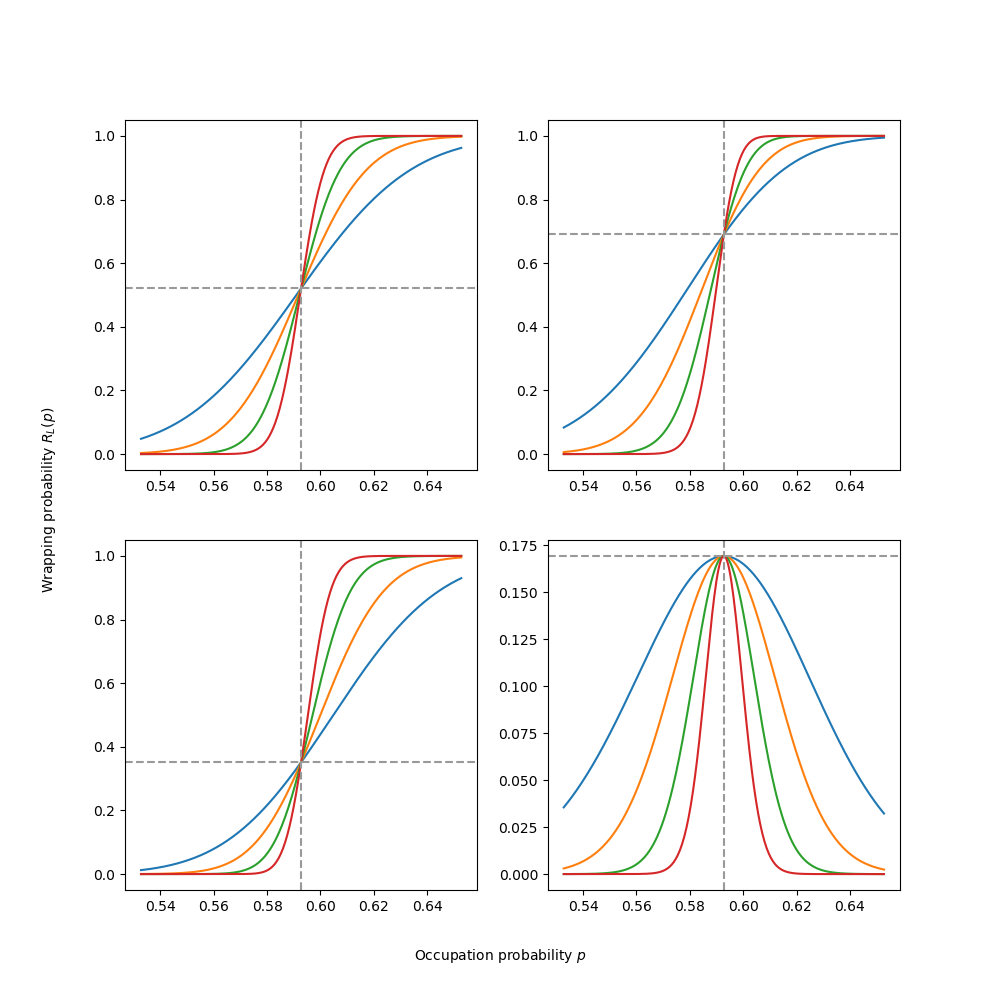
\includegraphics[width=\linewidth]{../plots/plot1}
		\caption{\label{fig:plot1} Plots of the wrapping probability functions $R_L(p)$ for (blue) $L=32$, (orange) $L=64$, (green) $L=128$, (red) $L=256$. The plots are zoomed on the region of critical percolation: (top left) $R_L^{(h)}$, (top right) $R_L^{(e)}$, (bottom left) $R_L^{(b)}$, (bottom right) $R_L^{(1)}$}
\end{figure}
\begin{figure}
	\centering
		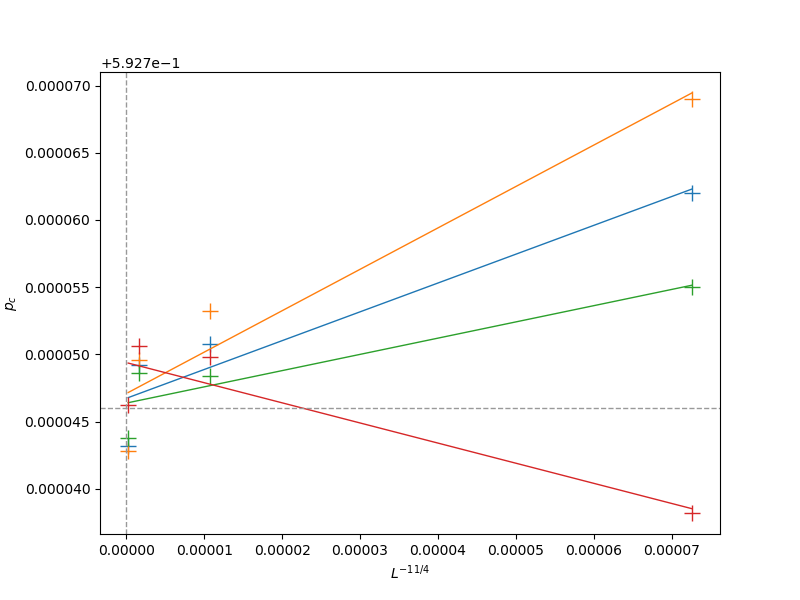
\includegraphics[width=0.9\linewidth]{../plots/plot2}
		\caption{\label{fig:plot2} Finite size scaling estimate for the critical percolation threshold. The colors correspond to the various wrapping probability definitions: (orange) $R_L^{(e)}$, (blue) $R_L^{(h)}$, (green) $R_L^{(b)}$, (red) $R_L^{(1)}$}
\end{figure}

\begin{table}[!htpb]
	\centering
		\begin{tabular}{ll}
		$R_L^{(h)}$ & 0.5927467(20) \\
		$R_L^{(e)}$ & 0.5927471(24) \\
		$R_L^{(b)}$ & 0.5927464(15) \\
		$R_L^{(1)}$ & 0.5927493(18)
		\end{tabular}
	\caption{\label{table:pc} The percolation threshold determined using the different wrapping probability functions: $R_L^{(h)}$ along the horizontal axis, $R_L^{(e)}$ along either axis, $R_L^{(b)}$ along both axes, $R_L^{(1)}$ along a single axis. }
\end{table}


\section{Conclusions and thoughts on further studies}
Despite its simplicity, the percolation problem displays many interesting properties, such as phase transition at the percolation threshold. We simulated finite lattices using the Newman-Ziff algorithm, which is efficient way to solve the problem. Finally, we estimated the value of the percolation threshold using finite size scaling. 

In the finite size estimation, we can see that the fit was quite poor due to the variance in the results. This is due to the lack of Monte Carlo samples, the number of which was heavily constrained by the time required to compute the simulation. A computation with more samples would yield an increased accuracy for the percolation threshold $p_c$. However, the computation duration was already in the order of tens of hours. Without parallelization and/or optimization, reproducing the results in~\cite{Newman_2001} would take weeks or months. Still, our results are in reasonable agreement with the state-of-the-art, and we can conclude that this is an excellent method to estimate the percolation threshold. 

Aside running the simulation longer, other interesting paths to take would be to simulate the system in higher dimensions, or on a different kind of lattice, such as a triangular lattice. A simulation in a continuum instead of a regular lattice would be interesting as well.











%
\clearpage
%\nocite{*}
%\addcontentsline{toc}{section}{\numberline{}References}

%%%%% If using BiBTeX, use the following two lines
\bibliographystyle{ieeetr}%unsrt
\bibliography{references}
%%%%% else if using \begin{thebibliography}{9}, use the following line
%\input{bibliography}
%%%%% endif
%
\clearpage
\appendix
\pagenumbering{Roman}
\setcounter{page}{1}
%
\section{The Newman-Ziff algorithm implemented in the C language}
\label{sect:appendixA}


\begin{minted}{c}


#include <stdlib.h>
#include <stdio.h>
#include <time.h>
#include <assert.h>
#include "mtwister.h"

/* Site percolation for square LxL lattice with
 periodic boundary conditions */

#define L 256 /* Linear dimension */
#define N (L*L)
#define EMPTY (-N-1)

#define STACKSIZE 100

#define MAX(a,b) ((a) > (b) ? (a) : (b))
#define MIN(a,b) ((a) < (b) ? (a) : (b))

/* 
For non-root occupied sites, contains the label 
for the site's parent in the tree
Root sites are marked with a negative value equal 
to minus the size of the cluster
For unoccupied states the value is EMPTY
*/
int ptr[N];          /* Array of pointers */

/*
Contains a list of the nearest neighbors, c
hange this to work with a different topology
*/
int nn[N][4];        /* Nearest neighbors */

/*
Contains the random occupation order  
*/
int order[N];        /* Occupation order */

/* Difference vector from the site to the cluster root */
int dx[N];
int dy[N];

/* Number of occupied sites in the 
configuration in which percolation first occurs */
int nx;
int ny;

/*
Sets up the nearest neighbors according to the chosen topology
periodical boundary conditions
*/
void boundaries()
{
    int i;

    for (i=0; i<N; i++) {
        nn[i][0] = (i+1)%N; /* Right */
        nn[i][1] = (i+N-1)%N; /* Left */
        nn[i][2] = (i+L)%N; /* Down */
        nn[i][3] = (i+N-L)%N; /* Up */
        if (i%L==0) nn[i][1] = i+L-1; /* First column */
        if ((i+1)%L==0) nn[i][0] = i-L+1; /* Last column */
    }
}

/*
Generates the random order in which the sites are occupied, 
randomly permuting the integers from 0 to N-1
*/
void permutation(MTRand *r)
{
    int i,j;
    int temp;

    for (i=0; i<N; i++) order[i] = i; 
    for (i=0; i<N; i++) {dx[i] = 0, dy[i] =0;}; 
    
    nx = 0;
    ny = 0;
    
    for (i=0; i<N; i++) {

        /* Permute the current integer with a randomly
         chosen integer from further in the list */
        double drand = genRand(r);
        j = i + (N-i)*drand;
        j = j % N;
        assert(0 <= drand && drand <= 1);
        assert(0 <= j && j < N);

        temp = order[i]; /* Swap i and j */
        order[i] = order[j];
        order[j] = temp;
    }
}

/* Finds the root pointer given a site 
and compresses the paths and displacements */
int findroot(int i)
{
    int r; /* Root */
    int sp=0; /* Stack pointer */
    int stack[STACKSIZE];

    /* Stack of displacements */
    int dx_s[STACKSIZE], dy_s[STACKSIZE];
    /* Cumulative displacement */ 
    int dx_cum = 0, dy_cum = 0;  

    r = i;

    while (ptr[r]>=0) {
        
        dx_s[sp] = dx[r];
        dy_s[sp] = dy[r];
        stack[sp] = r;
        r = ptr[r];
        sp++;
    }

    while (sp) {
        sp--;
        dx_cum += dx_s[sp];
        dy_cum += dy_s[sp];

        dx[stack[sp]] = dx_cum;
        dy[stack[sp]] = dy_cum;
        ptr[stack[sp]] = r;
    }
    return r;
}



/* Populate the lattice anc check for percolation */ 
void percolate()
{
    int i,j;
    int s1,s2;
    int r1,r2;
    
    for (i=0; i<N; i++) ptr[i] = EMPTY; 

    for (i=0; i<N; i++) {

        /* Occupy the next site randomly  */ 
        r1 = s1 = order[i]; 
        ptr[s1] = -1;       

        for (j=0; j<4; j++) {   
            s2 = nn[s1][j];     
            
            if (ptr[s2]!=EMPTY) { 
                r2 = findroot(s2);  
                
                /* Merge the clusters */
                if (r2!=r1) {               
                    if (ptr[r1]>ptr[r2]) {  
                        /* Increase the size of 
                        the amalgamated cluster */
                        ptr[r2] += ptr[r1]; 
                        
                        findroot(s1);
                        
                        ptr[r1] = r2;       
                        
                        /* Update the displacements */
                        findroot(s2);
                        dx[r1] = - dx[s1] + dx[s2];
                        dy[r1] = - dy[s1] + dy[s2];
                        
                        /* Unit vector between the two sites */
                        switch (j) {
                            case 0:
                                dx[r1] += + 1;    
                                break;
                            case 1:
                                dx[r1] += - 1;      
                                break;
                            case 2: 
                                dy[r1] += + 1;        
                                break;
                            case 3:  
                                dy[r1] += - 1;        
                                break;
                        }
                        

                        r1 = r2;

                    } else {
                        ptr[r1] += ptr[r2];
                        
                        findroot(s2);
                        
                        ptr[r2] = r1;

                        /* Update the displacements */
                        
                        findroot(s1);
                        dx[r2] = - dx[s2] + dx[s1];
                        dy[r2] = - dy[s2] + dy[s1];

                        /* Find the unit vector between 
                        the two sites */
                        switch (j) {
                            case 0:
                                dx[r2] += - 1;   
                                break;
                            case 1:
                                dx[r2] += + 1;  
                                break;
                            case 2:
                                dy[r2] += - 1;        
                                break;
                            case 3:
                                dy[r2] += + 1;        
                                break;
                        }
                        
                    }
                }
                else {
                /* Internal bond, therefore we can test
                 for percolation */

                    int dx1 = 0, dy1 = 0, dx2 = 0, dy2 = 0;

                    findroot(s1);
                    findroot(s2);
                    dx1 = dx[s1];
                    dx2 = dx[s2];
                    dy1 = dy[s1];
                    dy2 = dy[s2];

                    /* Unit vector of the newly added bond */
                    switch (j) {
                        case 0:
                            dx1 += -1;   
                            break;
                        case 1:
                            dx1 += +1;  
                            break;
                        case 2:
                            dy1 += -1;        
                            break;
                        case 3:
                            dy1 += +1;        
                            break;
                    }

                    /* Check for a multiply connected cluster */
                    if (!nx && abs(dx1-dx2) != 0) {
                        nx = i+1;
                    }
                    if (!ny && abs(dy1-dy2) != 0) {
                        ny = i+1;
                    }

                    /* Stop the calculation when percolation has
                    occurred in both axis */
                    if (nx && ny)
                        return;
                }
            }
        }
    }

    /* Should never happen since the system percolates
    always before all the sites are occupied */
    return;
}


int main()
{

    /* Number of Monte Carlo samples */
    int NUM_SIM = 1e7;

    /* Pseudo-random number generator*/
    MTRand r = seedRand(42);


    /* Percolation probabilities as a function 
    of the number of occupied sites */
    int RLh[N], RLb[N];
    for (int i = 0; i< N; i++) {
        RLh[i] = 0;
        RLb[i] = 0;
    }
    
    /* Simulation */
    boundaries();
    for (int j = 0; j < NUM_SIM; j++) {
        permutation(&r);
        percolate();

        for (int i = nx-1; i < N; i++)
                RLh[i] += 1;
        for (int i = MAX(nx-1, ny-1); i < N; i++)
                RLb[i] += 1;
    }

    /* Print the probabilities into std output*/
    for (int i = 0; i < N; i++) {
        printf("%i %.17g %.17g\n", i+1, 
            (double)RLh[i] / NUM_SIM, 
            (double)RLb[i] / NUM_SIM);
    }
}

\end{minted}
%
\end{document}
